\documentclass[MachineLearning]{subfiles}
\begin{document}

%@@@@@@@@@@@@@@@@@@@@@@@@@@@@@@
% summarizes lecture 5
% author: Benjamin Ellenberger

\section{Classification}
Classification in general is the problem of identifying to which of a set of categories (sub-populations) a new observation belongs, on the basis of a training set of data containing observations (or instances) whose category membership is known. An example would be assigning a given email into "spam" or "non-spam" classes or assigning a diagnosis to a given patient as described by observed characteristics of the patient (gender, blood pressure, presence or absence of certain symptoms, etc.).
\\\\
Classification is considered an instance of supervised learning, i.e. learning where a training set of correctly identified observations is available. The corresponding unsupervised procedure is known as clustering, and involves grouping data into categories based on some measure of inherent similarity or distance.
\subsection{The problem of statistical decisions}
n objects should be grouped in the classes \(\printlatex{1,\ldots,k,\mathcal{D},\mathcal{O}}\).
\begin{itemize}
\item $\mathcal{D}$: doubt class (more measurements required)
\item $\mathcal{O}$: outlier class (definitely none of the classes \(\printlatex{1,\ldots,k}\))
\end{itemize}
\textbf{Objects:} are characterized by feature vectors \(\printlatex{X \in \mathcal{X}}\)(feature space).\\
\textbf{Feature space:} \(\printlatex{\mathcal{X} (= \mathcal{X}_1 \times \mathcal{X}_2 \times \ldots \times \mathcal{X}_d\text{ with }\mathcal{X}_i \subseteq \R) \subset \R^d}\)\\
\textbf{Feature vector X:} \(\printlatex{\mathcal{O} \rightarrow \R^d \times \underbrace{[1,\ldots,k]}_{classes}}\)\\
\(\printlatex{\textit{o} \rightarrow (X_0,Y_0)}\)\\
Data \(\printlatex{\mathcal{Z}}\): \(\printlatex{\{(x_i,y_i) : 1 \leq i \leq n\}}\)
\todo[inline]{Use consistent notation: \(\mathcal{O}\) stands for outlier class and for the object space at the same time.}
\subsection{Bayesian Decision Theory}
The methods of statistical inference previously described are often referred to as classical methods. Bayesian methods (so called after the English mathematician Thomas Bayes) provide alternatives that allow one to combine prior information about a population parameter with information contained in a sample to guide the statistical inference process. A prior probability distribution for a parameter of interest is specified first. Sample information is then obtained and combined through an application of Bayes’s theorem to provide a posterior probability distribution for the parameter. The posterior distribution provides the basis for statistical inferences concerning the parameter. A key, and somewhat controversial, feature of Bayesian methods is the notion of a probability distribution for a population parameter. According to classical statistics, parameters are constants and cannot be represented as random variables. Bayesian proponents argue that, if a parameter value is unknown, then it makes sense to specify a probability distribution that describes the possible values for the parameter as well as their likelihood. The Bayesian approach permits the use of objective data or subjective opinion in specifying a prior distribution. With the Bayesian approach, different individuals might specify different prior distributions. Classical statisticians argue that for this reason Bayesian methods suffer from a lack of objectivity. Bayesian proponents argue that the classical methods of statistical inference have built-in subjectivity (through the choice of a sampling plan) and that the advantage of the Bayesian approach is that the subjectivity is made explicit.\\\\
Bayesian methods have been used extensively in statistical decision theory (see below Decision analysis). In this context, Bayes’s theorem provides a mechanism for combining a prior probability distribution for the states of nature with sample information to provide a revised (posterior) probability distribution about the states of nature. These posterior probabilities are then used to make better decisions.\\\\
\textbf{Bayes’s theorem}
Bayes’s theorem is in probability theory a means for revising predictions in light of relevant evidence, also known as conditional probability or inverse probability. The theorem was discovered among the papers of the English Presbyterian minister and mathematician Thomas Bayes and published posthumously in 1763. Related to the theorem is Bayesian inference, or Bayesianism, based on the assignment of some a priori distribution of a parameter under investigation. In 1854 the English logician George Boole criticized the subjective character of such assignments, and Bayesianism declined in favour of confidence intervals and hypothesis tests, now basic research methods.
\subsubsection{Problem Setting for Bayesian Inference}
\textbf{Bayesian view:} Both feature vector X and class label Y of an
object O are random variables!\\
\textbf{Notation:}\\
\(\printlatex{\pi_y}\) : fraction of the samples out of class Y = y
(\(\printlatex{\pi_y}\) is known)\\
\(\printlatex{p_y (x) := P\{X = x|Y = y\}}\): probability distribution / density of the samples out of class Y = y (class conditional density)
\begin{enumerate}
\item \(\printlatex{p_y (x)}\) is unknown \(\printlatex{\rightarrow}\) density estimation
\item \(\printlatex{p_y (x)}\) is known up to a parameter \(\printlatex{\rightarrow}\) parameter estimation
\end{enumerate}
\textbf{Bayes rule:} \(\printlatex{\underbrace{P\{model|data\}}_{\text{posterior}} = \frac{\overbrace{P\{data|model\}}^{\text{likelihood}}\overbrace{P\{model\}}^{\text{prior}}}{\underbrace{P\{data\}}_{\text{evidence}}}}\)
\begin{itemize}
\item \(\printlatex{\overbrace{P\{model\}}^{\text{prior}}}\): This indicates one's previous estimate of the probability that a hypothesis is true, before gaining the current evidence.
\item \(\printlatex{\overbrace{P\{data|model\}}^{\text{likelihood}}}\): It indicates the compatibility of the evidence with the given hypothesis.
\item \(\printlatex{\underbrace{P\{model|data\}}_{\text{posterior}}}\): This tells us what we want to know: the probability of a hypothesis given the observed evidence.
\item \(\printlatex{\underbrace{P\{data\}}_{\text{evidence}}}\): It is the probability of the data being observed at all.
\item the quotient \(\printlatex{\frac{P(model|data)}{P(data)}}\) represents the support the data provides for the model.
\end{itemize}
\subsection{Bayesian Classifier}
Assume that we know how the features are distributed for the different classes, i.e., the class conditional densities p y (x) and their parameters are known.
What is the best classification strategy in this situation?
\[\printlatex{\hat c: \mathcal{X} \rightarrow \hat c(X) \rightarrow \mathcal{Y} := \{1,\ldots,k,\mathcal{D}\}}\] (Mapping of \(\printlatex{\mathcal{X}}\) into \(\printlatex{\mathcal{Y}}\). No outlier class)\\
\subsubsection{Classification error}
But we must minimize the classification error.\\\\
\[\printlatex{\hat{\mathcal{R}} ( \hat c | \mathcal{Z}) =
\sum\limits_{x \in \mathcal{X}} \I_{\{\hat c(x)\neq y\}} = \sum\limits_{(x_i,y_i) \in \mathcal{Z}}\I_{\{\hat c (x_i) \neq y_i \}} }\]
Note that this error count is a random variable!
Expected errors are also called the expected risk and they
define the quality of a classifier
\[\printlatex{\mathcal{R}(\hat c) = \sum\limits_{y\leq k} P(y)\E_{P(x|y)} \I_{\{\hat c (x)\neq y} |Y = y] + \text{terms from D}}\]
\subsubsection{Loss function}
Weighted mistakes are introduced when classification errors are not equally costly.
We introduce a loss function \(\printlatex{L(y, z)}\) which denotes the loss
for the decision z if class y is correct. Classification costs can also be asymmetric, that means \(\printlatex{L(y, z) \neq L(z, y)}\) (Think of one class having worse outcomes than the other).\\
Example for Loss functions is the \(\printlatex{L^{0-1}(y,z)}\) function.

\[\printlatex{L^{0-1}(y,z) = 
\begin{cases}
0 &\mbox{if } z = y \\ 
1 &\mbox{if } z \neq y \wedge z \neq D \text{ (wrong decision)}\\ 
d &\mbox{if } z = D \text{ (no decision)}
\end{cases}}\]
with according expected loss:
\[\printlatex{\mathcal{R}(\hat c , y) = \E_X [L^{0-1} (y, \hat c (x))|Y = y]
= \underbrace{P\{\hat c (x) = y \wedge \hat c (x) = D|Y = y\}}_{\text{pmc(y) probability of misclassification}} + \underbrace{d \cdot P\{\hat c (x) = D|Y = y\}}_{\text{pd(y) probability of doubt}}}\]
or in an general version
\[\printlatex{\mathcal{R}(\hat c ) = \sum\limits_{z \leq k}\overbrace{\pi_z}^{\hidewidth= P(Z = z)\hidewidth}  pmc(z) + d \cdot \sum\limits_{z \leq k}\pi_z pd(z) = \E_C[\mathcal{R}(\hat c , C)]}\]
\subsubsection{Posterior class probability}
\[\printlatex{\overbrace{p(y|x) \equiv P\{Y = y|X = x\}}^{Posterior} = \frac{\overbrace{\pi_y}^{\hidewidth Prior\hidewidth} \overbrace{p_y (x)}^{\hidewidth Likelihood\hidewidth}}{\underbrace{\sum_z \pi_z p_z (x)}_{Evidence}}}\]
\begin{itemize}
\item Prior: \(\printlatex{\pi_y := P(Y = y)}\) is the probability of class \(\printlatex{Y = y}\).
\item Likelihood: The class conditional density \(\printlatex{p_y (x)}\) is the
probability of observing data \(\printlatex{X = x}\) given class
\(\printlatex{Y = y}\) (= \(\printlatex{P\{X=x|Y=y\}}\)).
\end{itemize}
\subsubsection{Bayes classifier}
\textbf{General principle of the Bayes classifier:}Select the class \(\printlatex{y^{MAP}}\) with highest \(\printlatex{\pi_y p_y (x)}\) value if the costs for not making a decision exceed the loss of this class y MAP , i.e., \(\printlatex{\pi_y p_y (x) > (1 - d)p(x)}\).

Classification rule for \(\printlatex{L^{0- 1}}\) loss is:
\[\printlatex{
c(x) =
\begin{cases}
y & \mbox{if } p(y|x) = \max\limits_{z \leq k} p(z|x) > 1 - d,\\
D & \mbox{if } p(y|x) \leq 1 - d \forall y.
\end{cases}
}\]
Generalization to arbitrary loss functions:
\[\printlatex{
c(x) =
\begin{cases}
y & \mbox{ if } \sum\limits_z L(z, y)p(z|x) = \min\limits_{\rho\leq k} \sum\limits_z L(z, \rho)p(z|x) \leq d\\
D & else .
\end{cases}
}\]
\textbf{Remark on Outliers:}
The outlier concept causes conceptual problems and it does not fit to the statistical decision theory since outliers indicate an erroneous or incomplete specification of the statistical model! But for completeness:
\[\printlatex{\pi_\mathcal{O} p_\mathcal{O} (x) \geq \max\left\{(1 - d)p(x), \max\limits_z \pi_z p_z (x)\right\}}\]
\subsection{Discriminant functions}
Discriminant functions take the feature vector as an input and decide if the object belongs to their class. The highest output of a discriminant function \(\printlatex{g_c}\) makes the object belong to class c: \(\printlatex{\forall z\neq y:~g_c(x) > g_z(x) \Rightarrow \text{class c} }\). The classifier is said
to assign a feature vector \(x\) to class \(\printlatex{\omega_i}\) if
\[\printlatex{g_i (x) > g_j (x)}~\text{for all } j=i\]

Thus, the classifier is viewed as a network or machine that computes c discriminant
functions and selects the category corresponding to the largest discriminant.
\begin{figure}[H]
\centering
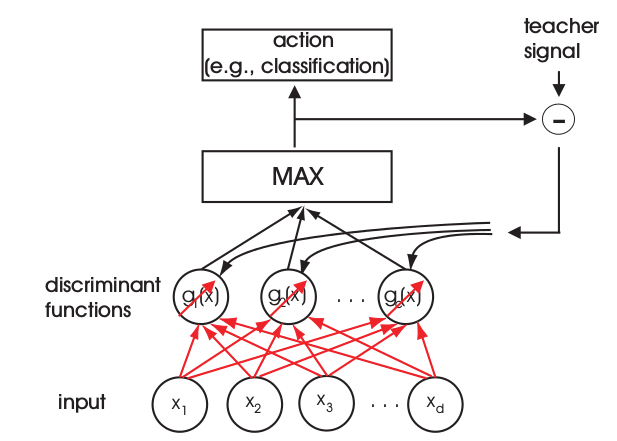
\includegraphics[width=0.47\linewidth]{figs/Adaptive-Discriminant-functions.png}
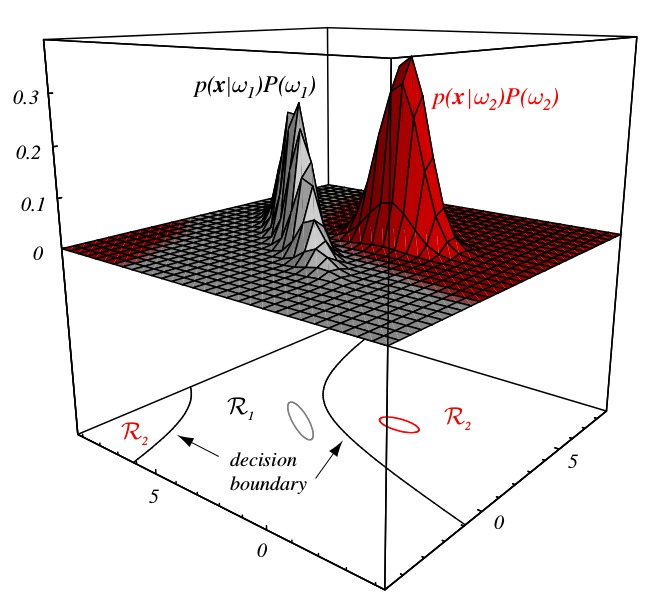
\includegraphics[width=0.47\linewidth]{figs/DF-decision-boundaries.png}
\caption{The red connections (weights) are adapted in such a way that the
teacher signal is imitated by the discriminant function. Source: Duda}
\end{figure}
\subsubsection{Linear classifiers}
We use normal distributions to describe the likelihood of class y:
\[\printlatex{p_y(x) = \frac{1}{\sqrt{2\pi^d|\underbrace{\Sigma_y}_{\hidewidth\text{Covariance matrix for class y}\hidewidth}|}}exp(-\frac{1}{2}(x-\mu_y)^T\Sigma^{-1}_y(x-\mu_y))}\]
Linear classifiers have a linear decision rule: 
\begin{align}
w^T (x - x_0) &= 0\\
w &= \mu_{y1}-\mu_{y2}\\
x_0 &= \frac{1}{2}(\mu_{y1}+\mu_{y2}) - \frac{\sigma^2w}{||w||^2} \log\frac{\pi_{y1}}{\pi_{y2}}
\end{align} 
The separating hyperplane is defined by the difference vector w and the offset \(\printlatex{x_0}\). The hyperplane is shifted by the log prior relative to the average of the two means.
\begin{figure}
\centering
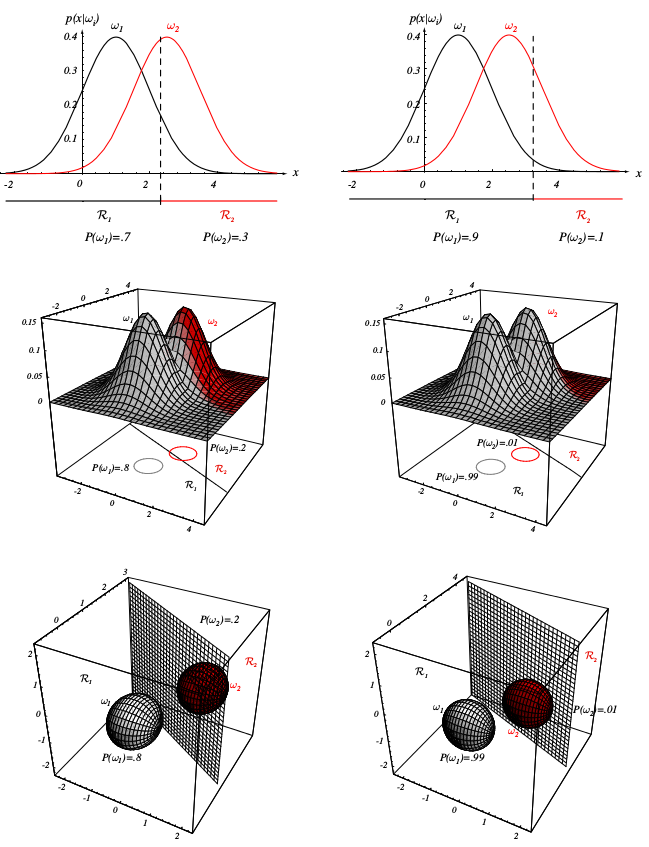
\includegraphics[width=0.7\linewidth]{figs/Gaussian-decision-surface.png}
\caption{If the covariance matrices for two distributions are equal and proportional to the identity matrix, then the distributions are spherical in d dimensions, and the boundary is a generalized hyperplane of d - 1 dimensions perpendicular to functions the line separating the means. In these one-, two-, and three-dimensional examples, we indicate \(\protect\printlatex{p (x|\omega_i)}\) and the boundaries for the case \(\protect\printlatex{P(\omega_1) = P(\omega_2)}\). In the three-dimensional case, the grid plane separates \(\protect\printlatex{\mathcal{R}_1}\) and \(\protect\printlatex{\mathcal{R}_2}\). The prior can cause a significant shift of the linear discriminant function in the direction of the less probable mode. Strong priors might even shift the linear discriminant function beyond the mode peak of the alternative class (see right column).}
\end{figure}
\paragraph{Generalized linear classifier \(\protect\printlatex{\Sigma_y = \Sigma \forall y}\)}
\begin{align}
w^T (x - x_0) &= 0\\
w &= \Sigma^{-1}(\mu_{y1}-\mu_{y2})\\
x_0 &= \frac{1}{2}(\mu_{y1}+\mu_{y2}) - \frac{\mu_{y1}-\mu_{y2}}{\underbrace{(\mu_{y1}-\mu_{y2})^T w}_{\text{Mahalanobis distance}}} \log\frac{\pi_{y1}}{\pi_{y2}}
\end{align}
\todo[inline]{How much detail is important here?}

\subsection{Readings}
\begin{enumerate}
\item Duda 2ed., Chapter 2,Bayesian Decision Theory (2.1,2.2,2.3.2,2.4,2.5,2.6)
\end{enumerate}
\todo[inline]{Write readings separately for all topics of classification.}
\end{document}